\documentclass[tikz,border=8pt]{standalone}
\usepackage[scaled=0.95]{helvet}
\renewcommand{\familydefault}{\sfdefault}
\usetikzlibrary{arrows.meta}
\definecolor{TEJNavy}{HTML}{1E2B55}
\definecolor{TEJBlue}{HTML}{1769AA}
\definecolor{TEJRed}{HTML}{B3261E}
\definecolor{TEJGold}{HTML}{B8860B}
\begin{document}
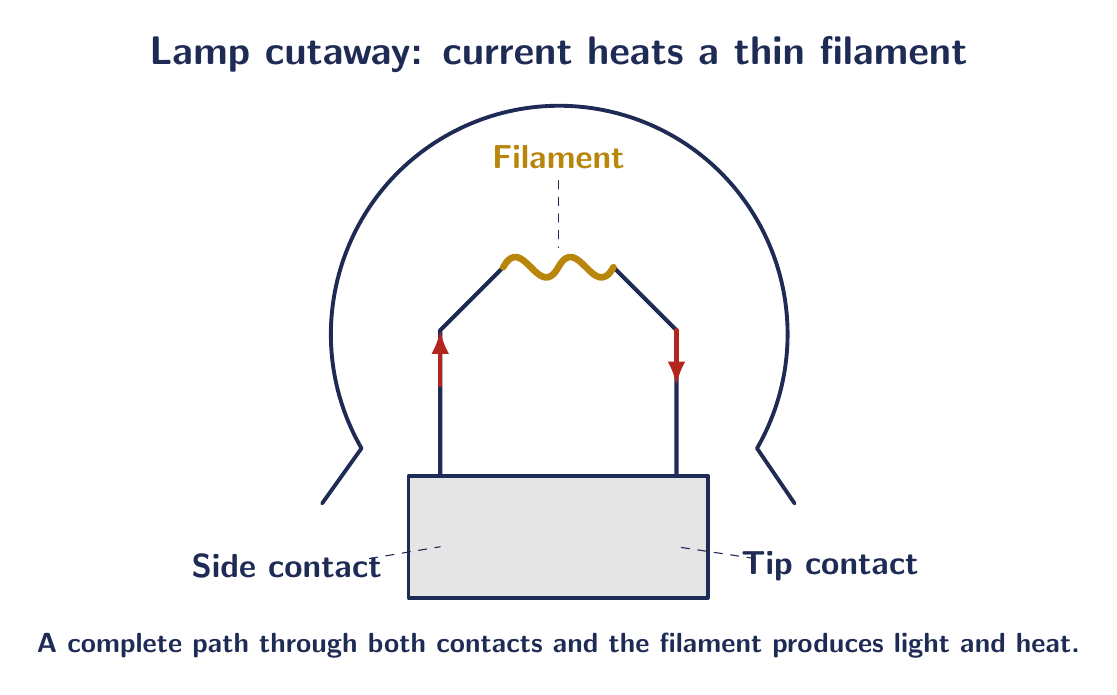
\begin{tikzpicture}[line cap=round,line join=round,font=\sffamily]
  \draw[TEJNavy,line width=1.4pt] (2,0.8) -- (2.5,1.5) arc[start angle=210,end angle=-30,radius=2.9] -- (8,0.8);
  \filldraw[fill=black!10,draw=TEJNavy,line width=1.2pt] (3.1,-0.4) rectangle (6.9,1.15);
  \draw[TEJNavy,line width=1.5pt] (3.5,1.15) -- (3.5,3.0) -- (4.3,3.8);
  \draw[TEJNavy,line width=1.5pt] (6.5,1.15) -- (6.5,3.0) -- (5.7,3.8);
  \draw[TEJGold,line width=2.4pt] (4.3,3.8) .. controls (4.55,4.25) and (4.75,3.35) .. (5.0,3.8) .. controls (5.25,4.25) and (5.45,3.35) .. (5.7,3.8);
  \node[font=\bfseries\Large,text=TEJNavy] at (5,6.5) {Lamp cutaway: current heats a thin filament};
  \node[font=\bfseries\large,text=TEJGold] at (5,5.2) {Filament};
  \draw[TEJNavy,dashed] (5,4.9) -- (5,4.05);
  \node[font=\bfseries\large,text=TEJNavy] at (1.55,0) {Side contact};
  \node[font=\bfseries\large,text=TEJNavy] at (8.45,0) {Tip contact};
  \draw[TEJNavy,dashed] (2.6,0.1) -- (3.5,0.25);
  \draw[TEJNavy,dashed] (7.5,0.1) -- (6.5,0.25);
  \draw[-{Latex[length=3mm]},TEJRed,line width=1.5pt] (3.5,2.3) -- (3.5,3.0);
  \draw[-{Latex[length=3mm]},TEJRed,line width=1.5pt] (6.5,3.0) -- (6.5,2.3);
  \node[font=\bfseries,text=TEJNavy,align=center] at (5,-1.0) {A complete path through both contacts and the filament produces light and heat.};
\end{tikzpicture}
\end{document}
